\mychapter{1}{Assignment 5 \\ \vspace{-0.3cm} Building Machine Learning Models
with Scikit-learn}
\addcontentsline{toc}{chapter}{Assignment 5 Building Machine Learning Models
with Scikit-learn}
\usepackage{graphicx}


\section*{Problem Statement 1:Classification on the Iris Dataset}



\begin{enumerate}
    \item  Load the Iris dataset from Seaborn’s dataset module into a Pandas DataFrame.
    \item Split the dataset into training and test data.
    \item Train and evaluate the following classification models:
        \begin{enumerate}
        \item  K-Nearest Neighbors (KNN).
        \item Gaussian Naive Bayes.
        \item Decision Tree.
        \item Random Forest
        \item Support Vector Machine (SVM)
       \end{enumerate}
    \item For each model:
     \begin{enumerate}
        \item  Print the labels predicted by the model on the test data and compare them with
the actual labels.
        \item Form and display the confusion matrix using the test data.
       
    \end{enumerate}
    \section*{Problem Statement 2: K-Means Clustering on the Wine Dataset}



    \item  Load the Wine dataset from Scikit-learn’s dataset module into a Pandas DataFrame.
    \item Preprocess the data by selecting relevant features and handling any missing values
if present.
    \item Apply K-Means clustering to the dataset with the number of clusters equal to the
number of unique wine classes in the dataset.
    \item Print the cluster labels assigned to each data point by the K-Means algorithm.
    \item Compare the cluster labels with the actual wine class labels by calculating the accuracy of the clustering.
    \item Visualize the clusters using a scatter plot or pairplot with different colors representing different clusters.
        \section*{Problem Statement 3: Linear Regression on the California Housing Dataset}


    \item Load the California Housing dataset from Scikit-learn’s dataset module into a Pandas
DataFrame.
    \item Preprocess the data by selecting relevant features and handling any missing values
if present.
    \item Split the dataset into training and test data.
    \item Train a Linear Regression model on the training data.
    \item Evaluate the model by predicting housing prices on the test data and calculating
performance metrics such as Mean Squared Error (MSE) and R-squared.
   \item Print the coefficients of the model to understand the influence of each feature on the
target variable.
    
\end{enumerate}

\newpage

\vspace{-.15cm}
\section{Loading the Dataset}
\vspace{-.75cm}
\begin{code}
\begin{lstlisting}
import seaborn as sns
import pandas as pd
iris = sns.load_dataset('iris')
df = pd.DataFrame(iris)
print(df.head())
\end{lstlisting}
\end{code}
\vspace{-1cm}
\begin{verbatim} 
   sepal_length  sepal_width  petal_length  petal_width species
0           5.1          3.5           1.4          0.2  setosa
1           4.9          3.0           1.4          0.2  setosa
2           4.7          3.2           1.3          0.2  setosa
3           4.6          3.1           1.5          0.2  setosa
4           5.0          3.6           1.4          0.2  setosa

[ ]

\end{verbatim}
\vspace{-.6cm}
\section{ Split the Dataset}
\vspace{-.75cm}
\begin{code}
\begin{lstlisting}
 from sklearn.model_selection import train_test_split
train_df, test_df = train_test_split(df, test_size=0.2)
print("train data \n",train_df.head())
print("test data \n",test_df.head())
\end{lstlisting}
\end{code}
\vspace{-1cm}
\begin{verbatim}
train data 
      sepal_length  sepal_width  petal_length  petal_width     species
108           6.7          2.5           5.8          1.8   virginica
0             5.1          3.5           1.4          0.2      setosa
46            5.1          3.8           1.6          0.2      setosa
105           7.6          3.0           6.6          2.1   virginica
87            6.3          2.3           4.4          1.3  versicolor
test data 
      sepal_length  sepal_width  petal_length  petal_width     species
137           6.4          3.1           5.5          1.8   virginica
97            6.2          2.9           4.3          1.3  versicolor
13            4.3          3.0           1.1          0.1      setosa
3             4.6          3.1           1.5          0.2      setosa
93            5.0          2.3           3.3          1.0  versicolor
\end{verbatim}

\vspace{-.3cm}
\section{Load the Wine Dataset}
\vspace{-.9cm}
\begin{code}
\begin{lstlisting}
X = df.drop('species', axis=1)
y = df['species']
import pandas as pd
from sklearn.metrics import confusion_matrix, accuracy_score
import seaborn as sns
import matplotlib.pyplot as plt
from sklearn.neighbors import KNeighborsClassifier
from sklearn.naive_bayes import GaussianNB
from sklearn.tree import DecisionTreeClassifier
from sklearn.ensemble import RandomForestClassifier
from sklearn.svm import SVC

def evaluate_model(model, X_test, y_test):
  y_pred = model.predict(X_test)
  print("Predicted Labels:")
  print(y_pred)
  print("Actual Labels:")
  print(y_test)

  cm = confusion_matrix(y_test, y_pred)
  print(cm)
  accuracy = accuracy_score(y_test, y_pred)
  print(f"Accuracy: {accuracy}")

knn = KNeighborsClassifier(n_neighbors=5)
knn.fit(X_train, y_train)
print("K-Nearest Neighbors:")
evaluate_model(knn, X_test, y_test)

nb = GaussianNB()
nb.fit(X_train, y_train)
print("Gaussian Naive Bayes:")
evaluate_model(nb, X_test, y_test)

dt = DecisionTreeClassifier()
dt.fit(X_train, y_train)
print("Decision Tree:")
evaluate_model(dt, X_test, y_test)

rf = RandomForestClassifier()
rf.fit(X_train, y_train)
print("Random Forest:")
evaluate_model(rf, X_test, y_test)

 svm = SVC()
svm.fit(X_train, y_train)
print("Support Vector Machine:")
evaluate_model(svm, X_test, y_test)   
\end{lstlisting}
\end{code}
\newpage
\vspace{-1cm}
\begin{verbatim}
K-Nearest Neighbors:
Predicted Labels:
['versicolor' 'setosa' 'virginica' 'versicolor' 'versicolor' 'setosa'
 'versicolor' 'virginica' 'versicolor' 'versicolor' 'virginica' 'setosa'
 'setosa' 'setosa' 'setosa' 'versicolor' 'virginica' 'versicolor'
 'versicolor' 'virginica' 'setosa' 'virginica' 'setosa' 'virginica'
 'virginica' 'virginica' 'virginica' 'virginica' 'setosa' 'setosa']
Actual Labels:
73     versicolor
18         setosa
118     virginica
78     versicolor
76     versicolor
31         setosa
64     versicolor
141     virginica
68     versicolor
82     versicolor
110     virginica
12         setosa
36         setosa
9          setosa
19         setosa
56     versicolor
104     virginica
69     versicolor
55     versicolor
132     virginica
29         setosa
127     virginica
26         setosa
128     virginica
131     virginica
145     virginica
108     virginica
143     virginica
45         setosa
30         setosa
Name: species, dtype: object
[[10  0  0]
 [ 0  9  0]
 [ 0  0 11]]
Accuracy: 1.0
Gaussian Naive Bayes:
Predicted Labels:
['versicolor' 'setosa' 'virginica' 'versicolor' 'versicolor' 'setosa'
 'versicolor' 'virginica' 'versicolor' 'versicolor' 'virginica' 'setosa'
 'setosa' 'setosa' 'setosa' 'versicolor' 'virginica' 'versicolor'
 'versicolor' 'virginica' 'setosa' 'virginica' 'setosa' 'virginica'
 'virginica' 'virginica' 'virginica' 'virginica' 'setosa' 'setosa']
Actual Labels:
73     versicolor
18         setosa
118     virginica
78     versicolor
76     versicolor
31         setosa
64     versicolor
141     virginica
68     versicolor
82     versicolor
110     virginica
12         setosa
36         setosa
9          setosa
19         setosa
56     versicolor
104     virginica
69     versicolor
55     versicolor
132     virginica
29         setosa
127     virginica
26         setosa
128     virginica
131     virginica
145     virginica
108     virginica
143     virginica
45         setosa
30         setosa
Name: species, dtype: object
[[10  0  0]
 [ 0  9  0]
 [ 0  0 11]]
Accuracy: 1.0
Decision Tree:
Predicted Labels:
['versicolor' 'setosa' 'virginica' 'versicolor' 'versicolor' 'setosa'
 'versicolor' 'virginica' 'versicolor' 'versicolor' 'virginica' 'setosa'
 'setosa' 'setosa' 'setosa' 'versicolor' 'virginica' 'versicolor'
 'versicolor' 'virginica' 'setosa' 'virginica' 'setosa' 'virginica'
 'virginica' 'virginica' 'virginica' 'virginica' 'setosa' 'setosa']
Actual Labels:
73     versicolor
18         setosa
118     virginica
78     versicolor
76     versicolor
31         setosa
64     versicolor
141     virginica
68     versicolor
82     versicolor
110     virginica
12         setosa
36         setosa
9          setosa
19         setosa
56     versicolor
104     virginica
69     versicolor
55     versicolor
132     virginica
29         setosa
127     virginica
26         setosa
128     virginica
131     virginica
145     virginica
108     virginica
143     virginica
45         setosa
30         setosa
Name: species, dtype: object
[[10  0  0]
 [ 0  9  0]
 [ 0  0 11]]
Accuracy: 1.0
Random Forest:
Predicted Labels:
['versicolor' 'setosa' 'virginica' 'versicolor' 'versicolor' 'setosa'
 'versicolor' 'virginica' 'versicolor' 'versicolor' 'virginica' 'setosa'
 'setosa' 'setosa' 'setosa' 'versicolor' 'virginica' 'versicolor'
 'versicolor' 'virginica' 'setosa' 'virginica' 'setosa' 'virginica'
 'virginica' 'virginica' 'virginica' 'virginica' 'setosa' 'setosa']
Actual Labels:
73     versicolor
18         setosa
118     virginica
78     versicolor
76     versicolor
31         setosa
64     versicolor
141     virginica
68     versicolor
82     versicolor
110     virginica
12         setosa
36         setosa
9          setosa
19         setosa
56     versicolor
104     virginica
69     versicolor
55     versicolor
132     virginica
29         setosa
127     virginica
26         setosa
128     virginica
131     virginica
145     virginica
108     virginica
143     virginica
45         setosa
30         setosa
Name: species, dtype: object
[[10  0  0]
 [ 0  9  0]
 [ 0  0 11]]
Accuracy: 1.0
Support Vector Machine:
Predicted Labels:
['versicolor' 'setosa' 'virginica' 'versicolor' 'versicolor' 'setosa'
 'versicolor' 'virginica' 'versicolor' 'versicolor' 'virginica' 'setosa'
 'setosa' 'setosa' 'setosa' 'versicolor' 'virginica' 'versicolor'
 'versicolor' 'virginica' 'setosa' 'virginica' 'setosa' 'virginica'
 'virginica' 'virginica' 'virginica' 'virginica' 'setosa' 'setosa']
Actual Labels:
73     versicolor
18         setosa
118     virginica
78     versicolor
76     versicolor
31         setosa
64     versicolor
141     virginica
68     versicolor
82     versicolor
110     virginica
12         setosa
36         setosa
9          setosa
19         setosa
56     versicolor
104     virginica
69     versicolor
55     versicolor
132     virginica
29         setosa
127     virginica
26         setosa
128     virginica
131     virginica
145     virginica
108     virginica
143     virginica
45         setosa
30         setosa
Name: species, dtype: object
[[10  0  0]
 [ 0  9  0]
 [ 0  0 11]]
Accuracy: 1.0
\end{verbatim}

\vspace{-.75cm}
\section{ Preprocess the Data}
\vspace{-.6cm}
\begin{code}
\begin{lstlisting}
 from sklearn.datasets import load_wine
import pandas as pd

wine = load_wine()
df = pd.DataFrame(data=wine.data, columns=wine.feature_names)
df['target'] = wine.target
print(df.head())
\end{lstlisting}
\end{code}
\vspace{-.75cm}
\begin{verbatim}
    alcohol  malic_acid   ash  alcalinity_of_ash  magnesium  total_phenols  \
0    14.23        1.71  2.43               15.6      127.0           2.80   
1    13.20        1.78  2.14               11.2      100.0           2.65   
2    13.16        2.36  2.67               18.6      101.0           2.80   
3    14.37        1.95  2.50               16.8      113.0           3.85   
4    13.24        2.59  2.87               21.0      118.0           2.80   

   flavanoids  nonflavanoid_phenols  proanthocyanins  color_intensity   hue  \
0        3.06                  0.28             2.29             5.64  1.04   
1        2.76                  0.26             1.28             4.38  1.05   
2        3.24                  0.30             2.81             5.68  1.03   
3        3.49                  0.24             2.18             7.80  0.86   
4        2.69                  0.39             1.82             4.32  1.04   

   od280/od315_of_diluted_wines  proline  target  
0                          3.92   1065.0       0  
1                          3.40   1050.0       0  
2                          3.17   1185.0       0  
3                          3.45   1480.0       0  
4                          2.93    735.0       0
\end{verbatim}
\vspace{-.75cm}
\section{Apply K-Means Clustering}
\vspace{-.6cm}
\begin{code}
\begin{lstlisting}
df.isnull().sum()
df.dropna(inplace=True)
df.fillna(df.mean(), inplace=True)
from sklearn.feature_selection import SelectKBest, f_classif
selector = SelectKBest(f_classif, k=5)
X_new = selector.fit_transform(df.drop('target', axis=1), df['target'])
selected_features = df.drop('target', axis=1).columns[selector.get_support()]
df = df[selected_features]
df['target'] = wine.target
\end{lstlisting}
\end{code}
\vspace{-1cm}
\begin{verbatim}
 
                                0
alcohol	                        0
malic_acid	                     0
ash	                            0
alcalinity_of_ash	              0
magnesium	                      0
total_phenols	                  0
flavanoids	                     0
nonflavanoid_phenols        	   0
proanthocyanins             	   0
color_intensity             	   0
hue	                            0
od280/od315_of_diluted_wines	   0
proline	                        0
target	                         0
dtype: int64
\end{verbatim}
%\vspace{-.6cm}
%\newpage
\section{ Print Cluster Labels}
\begin{lstlisting}
from sklearn.cluster import KMeans

n_clusters = len(df['target'].unique())

kmeans = KMeans(n_clusters=n_clusters, random_state=42)

kmeans.fit(df.drop('target', axis=1))


labels = kmeans.labels_

df['cluster'] = labels
print(df.head())
df.to_csv('clustered_wine_data.csv', index=False)
\end{lstlisting}
\begin{verbatim}
    alcohol  flavanoids  color_intensity  od280/od315_of_diluted_wines  \
0    14.23        3.06             5.64                          3.92   
1    13.20        2.76             4.38                          3.40   
2    13.16        3.24             5.68                          3.17   
3    14.37        3.49             7.80                          3.45   
4    13.24        2.69             4.32                          2.93   

   proline  target  cluster  
0   1065.0       0        1  
1   1050.0       0        1  
2   1185.0       0        1  
3   1480.0       0        1  
4    735.0       0        0  
\end{verbatim}
\section{ Compare Cluster Labels with Actual Labels}
\begin{lstlisting}
print(df['cluster'])
\end{lstlisting}
\newpage
\begin{verbatim}
0      1
1      1
2      1
3      1
4      0
      ..
173    0
174    0
175    0
176    0
177    2
Name: cluster, Length: 178, dtype: int32                

\end{verbatim}
\section{Compare Cluster Labels with Actual Labels}
\begin{lstlisting}
print(accuracy_score(df['target'], df['cluster']))
\end{lstlisting}
\begin{verbatim}
 0.1853932584269663                

\end{verbatim}
\section{Visualize the Clusters}
\begin{lstlisting}
import seaborn as sns
import matplotlib.pyplot as plt

sns.pairplot(df, hue='cluster', palette='viridis')
plt.show()
\end{lstlisting}

\newpage

\begin{figure}[h!]
    \centering
    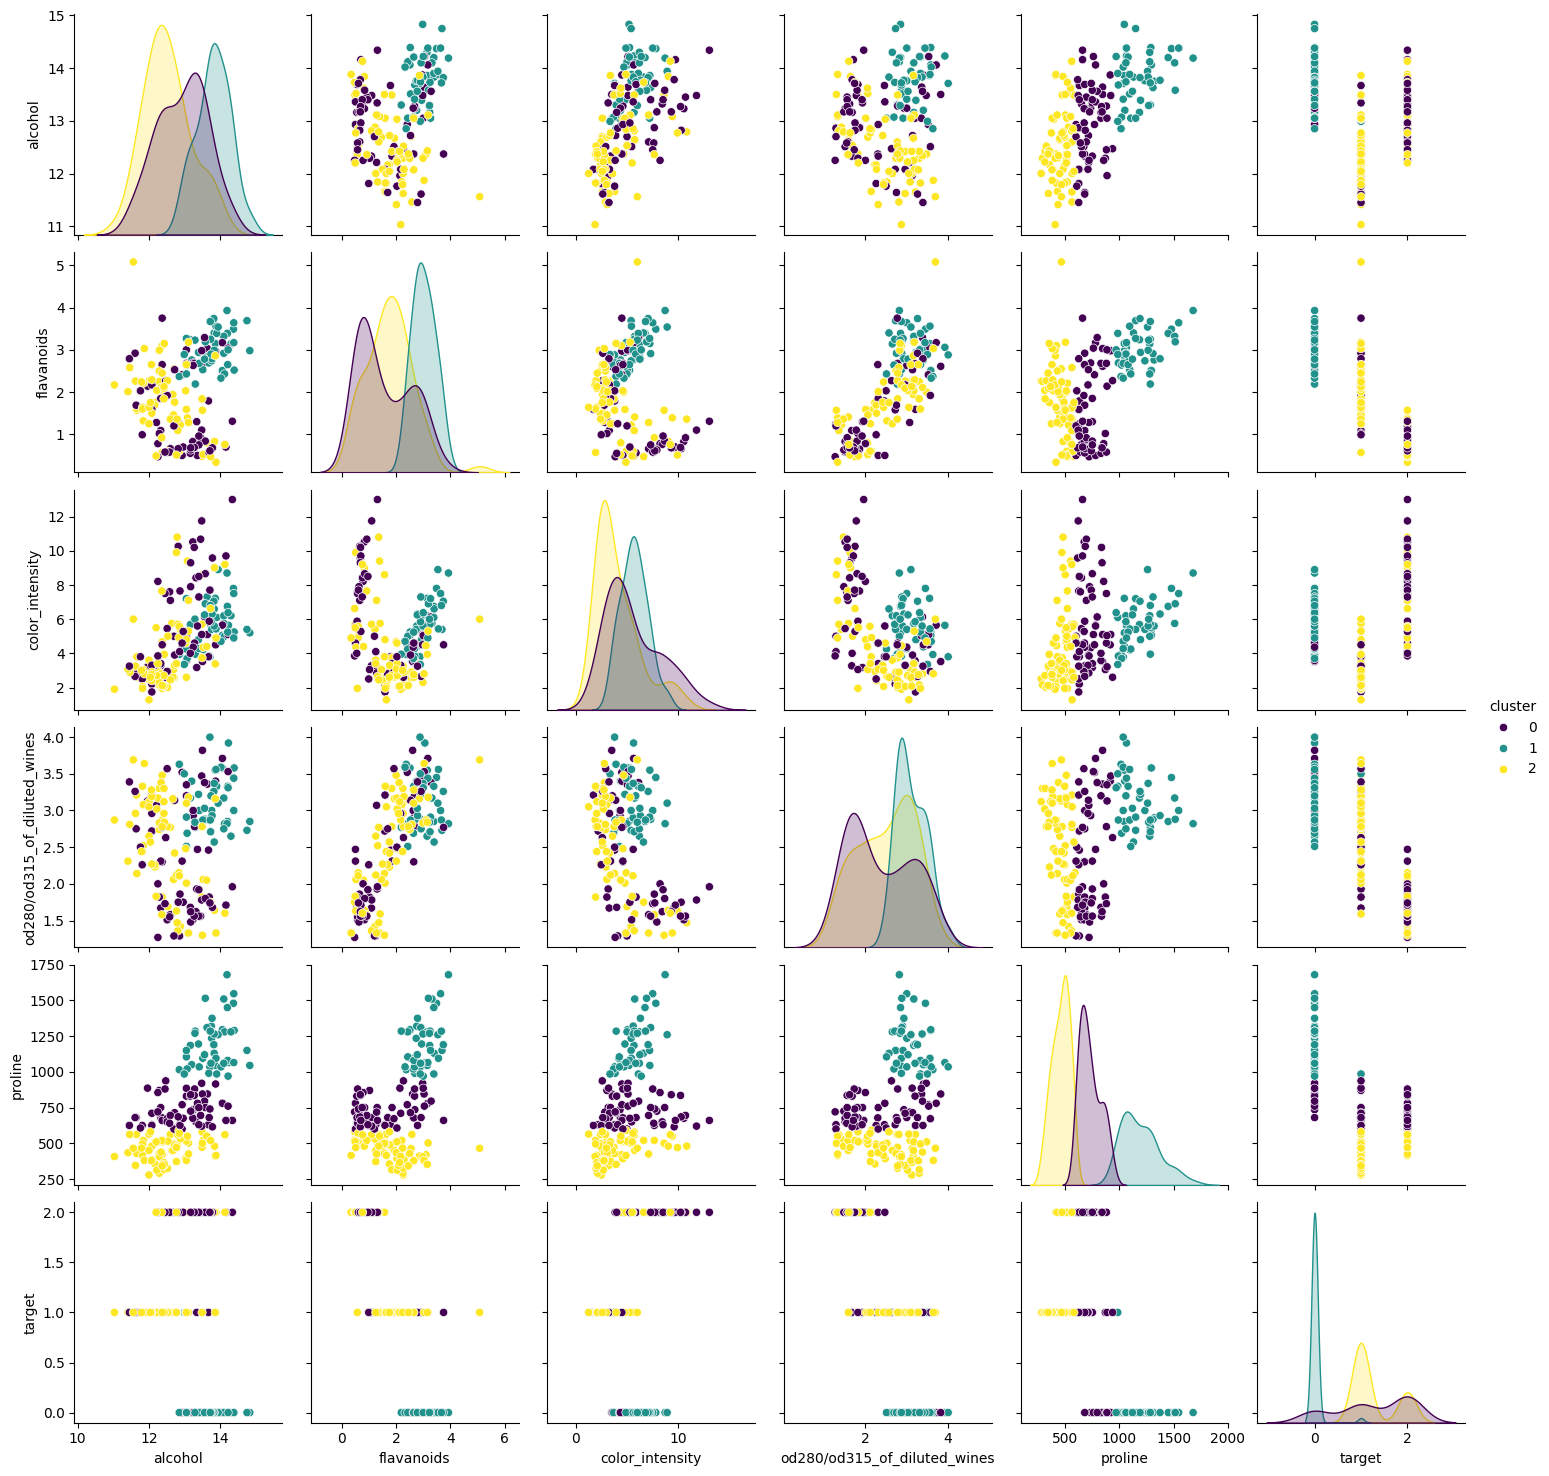
\includegraphics[width=0.8\textwidth]{download.png}
    \caption{}
     \label{}
\end{figure}            


\section*{Problem Statement 3: Linear Regression on the California Housing Dataset}
\section{ Load the California Housing Dataset}
\begin{lstlisting}
 from sklearn.datasets import fetch_california_housing 
import pandas as pd
housing = fetch_california_housing() 
df = pd.DataFrame(data=housing.data, columns=housing.feature_names) 
df['target'] = housing.target 
print(df.head()) 
\end{lstlisting}
\begin{verbatim}
    MedInc  HouseAge  AveRooms  AveBedrms  Population  AveOccup  Latitude  \ 
0  8.3252      41.0  6.984127   1.023810       322.0  2.555556     37.88    
1  8.3014      21.0  6.238137   0.971880      2401.0  2.109842     37.86    
2  7.2574      52.0  8.288136   1.073446       496.0  2.802260     37.85    
3  5.6431      52.0  5.817352   1.073059       558.0  2.547945     37.85    
4  3.8462      52.0  6.281853   1.081081       565.0  2.181467     37.85    
   Longitude  target   
0    -122.23   4.526   
1    -122.22   3.585   
2    -122.24   3.521   
3    -122.25   3.413   
4    -122.25   3.422   
\end{verbatim}
\section{Preprocess the Data}
\begin{lstlisting}
 df.isnull().sum() 
df.fillna(df.mean(), inplace=True) 
from sklearn.feature_selection import SelectKBest, f_regression 
selector = SelectKBest(f_regression, k=5)  
X_new = selector.fit_transform(df.drop('target', axis=1), df['target']) 
selected_features = df.drop('target', axis=1).columns[selector.get_support()] 
\end{lstlisting}
\section{Split the Dataset}
\begin{lstlisting}
    X_train, X_test, y_train, y_test = train_test_split(X_california, y_california, test_size=0.3, random_state=42)
\end{lstlisting}

\section{ Train a Linear Regression Model}
\begin{lstlisting}
 from sklearn.model_selection import train_test_split 
X = df.drop('target', axis=1) 
y = df['target'] 
X_train, X_test, y_train, y_test = train_test_split(X, y, test_size=0.2, random_s
 from sklearn.linear_model import LinearRegression 
model = LinearRegression() 
model.fit(X_train, y_train) 
\end{lstlisting}
\begin{verbatim}
▾ LinearRegression
 LinearRegression()        
\end{verbatim}
\section{Evaluate the Model}
\begin{lstlisting}
 from sklearn.metrics import mean_squared_error, r2_score 
y_pred = model.predict(X_test) 
mse = mean_squared_error(y_test, y_pred) 
r2 = r2_score(y_test, y_pred) 
print(f'Mean Squared Error: {mse}') 
print(f'R-squared: {r2}')
\end{lstlisting}
\begin{verbatim}
Mean Squared Error: 0.6382565441555921 
R-squared: 0.5129333248216971         
\end{verbatim}
\section{ Print the Coefficients}
\begin{lstlisting}
 print(f'Coefficients: {model.coef_}')
 print(df[['X3 distancetothenearestMRTstation','decimal_scaled']].head())
\end{lstlisting}
\begin{verbatim}
Coefficients: [ 0.53520156  0.01618449 -0.20927062  1.050567   -0.03105515] 
\end{verbatim}

  




